% !TeX root = main.tex
\section{FW-UAV Design for 3D Mapping}

The following are the given requirement

\begin{align*}
    \textup{Endurance} = 60 \, \textup{min} &&
    \textup{Area of operation} = 10 \, \textup{Km rad.} &&
    \textup{Cruise speed} = 20 \, \textup{m/s} \\
    \textup{Flying altitude} = 100 \, \textup{m (from ground)} &&
    \textup{Climb rate} = 2 \, \textup{m/s} &&
    \textup{Descent rate} = 2 \, \textup{m/s}
\end{align*}

It is assumed that these are the minimum values and with a greater budget these can be extended. It is assumed that some compromise on the area of operation (in terms of coverage area and not range) is acceptable.

% CONOPS
\subsection{CONOPS}

\textbf{CONOPS} of \emph{Concept of Operations} is the overview of the operations involved in the application of the Fixed Wing UAV (FW-UAV). The stages of operation are defined as

\begin{enumerate}
    \item \textbf{Take-off} from ground. It is preferred to have a hand launch mechanism for take-off (bungee launch at best). Runway takeoff UAVs are least preferred (too much arrangement required for them).
    \item \textbf{Climb} to the height of $100 \, m$ from ground. The climb rate is $2 \, m/s$.
    \item \textbf{Cruise} in the area for performing mapping. It is assumed that the UAV travels in straight lines (back and forth) from one end to another end (confined in a circle - of $10\, Km$ radius).
    \begin{itemize}
        \item It is possible to take multiple trials for covering the entire area.
        \item It is preferred to have an autonomous solution, where the path is programmed and the UAV follows it.
        \item A manual solution is only required as a backup.
    \end{itemize}
    \item \textbf{Descent} from $100\, m$ to the ground. The descent rate is $2 \, m/s$.
    \item \textbf{Landing} on the ground. The UAV will be at very low speeds when landing and can land on any grassland. It need not have a runway for landing (it doesn't even need wheels).
\end{enumerate}

The \textit{loitering} phase was not chosen because we decided on traveling (cruising) in straight lines, while taking turns. This is better if multiple views are required. Loitering can be chosen if the desired path is in form of expanding circles. 

However, there will be no \textit{aggressive flight maneuvers}, as the application does not desire it.

% Requirements
\subsection{Requirement Specifications}

The following can be considered the \emph{requirement specifications} for the starting of the design phase

\begin{itemize}
    \item \textbf{Operating velocity} can be the cruise speed of $20\,m/s$.
    \item \textbf{Range} can be assumed to be around $30\,Km$ (for traversals). This will depend on the sensor. Some sensors can work from far, while some will require close proximity (increasing traversal range).
    \item \textbf{Endurance} can be $60\,min$.
    \item \textbf{Payload} will be the cameras and/or LiDAR sensors (which will be used for 3D mapping). Usually, these will be well under $500\,gm$.
    \item \textbf{Wind} conditions will be around $5\,km/hr$ to $20\,km/hr$ \footnote{Weather data from \url{https://www.meteoblue.com/en/weather/historyclimate/}}. They will hardly be expected to go beyond $25\,km/hr$.
    \item \textbf{Altitude} will be around $100\,m$ from ground, and $1000\,m$ to $3000\,m$ from sea level (mostly will be under $1500\,m$ for most commercial applications).
    \item \textbf{Safety}: The UAV must be certified for surveillance and mapping standards, as well as human operation standards. It also must have regulatory compliance with GOI (Government of India) guidelines. The following can be noted \footnote{Main reference from \url{https://uavcoach.com/drone-laws-in-india/} and \url{https://digitalsky.dgca.gov.in/home}}
    \begin{itemize}
        \item The drone falls in the \emph{micro} category (weighing total of $250 \, g$ to $2 \, kg$).
        \item Drone must have GPS, flight data logging, RTH (Return-to-home), anti-collision light, RFID and SIM with NPNT (No Permission No Takeoff) compliant software, and ID plate.
    \end{itemize}
    \item \textbf{Maneuverability}: No agile maneuvers are needed. The drone will be oriented horizontally virtually always. Only turning maneuvers are needed.
\end{itemize}

% Market research
\subsection{Market Survey}

\subsubsection*{senseFly eBee X}

The senseFly eBee X fixed wing UAV is a hand-launched UAV suitable for mapping and surveillance applications. It is very mobile and convenient to use. 

The product can be found at \url{https://www.sensefly.com/drone/ebee-x-fixed-wing-drone/}. Its specifications were obtained from the comparison table and datasheet at the same website.

\begin{enumerate}
    \item \textit{Operating velocity}: It can cruise from $11\,m/s$ to $30\,m/s$. Comfortably within our $20\,m/s$ bounds.
    \item \textit{Range}: It has a standard flight range of $37\,km$ (maximum is $55\,km$). This is well over our $30\,km$ requirement.
    \item \textit{Endurance}: It can fly for up to $90\,min$. Our requirement is only for $60\,min$.
    \item \textit{Payload}: It will carry a camera as payload. The total weight will be around $1.3\,kg$ to $1.6\,kg$. It is very easy to carry around in a bagpack.
    \item \textit{Wind}: It can tolerate wind up to $46\,km/hr$ (well beyond our maximum of $25\,km/hr$).
    \item \textit{Altitude}: Its optimal altitude is $120\,m$, we only require $100\,m$.
    \item \textit{Safety}: The UAV will require additional safety certification for India. It is certified for Canada, EU and the USA.
\end{enumerate}

With the above specifications, the UAV almost exceeds our requirements. Choosing it should give very comfortable bounds, thereby allowing for greater needs in the future.
Price would be around \rupee~10,00,000 (including all accessories and carrying case, with extra batteries and ground stations). This UAV is shown in figure \ref{fig:ms-sf-ebee-x}.

It has a $116\,cm$ wingspan.


\subsubsection*{Delair UX11}

The Delair UX 11 fixed wing UAV is a compact hand-launched UAV suitable for mapping applications. The UAV has 3G and 4G capabilities giving it extended communication range and reducing the number of ground stations to one (receiver).

The product can be found at \href{https://delair.aero/delair-commercial-drones/professional-mapping-drone-delair-ux11/}{https://delair.aero/}. Its specifications were obtained from the datasheet at the same website. Some information is also taken from its Amazon product page.

\begin{enumerate}
    \item \textit{Operating velocity}: The UAV can cruise at speed upto $15\,m/s$. This is a little less than our $20\,m/s$ requirement.
    \item \textit{Range}: It has a range of $53\,km$. This is well over our $30\,km$ requirement.
    \item \textit{Endurance}: It can fly for up to $60\,min$, which our exact requirement.
    \item \textit{Payload}: It will not require any external payload as the cameras are built into the UAV body. The entire UAV weighs less than $1.5\,kg$.
    \item \textit{Wind}: It can tolerate wind up to $45\,km/hr$ (well beyond our maximum of $25\,km/hr$). It can even fly in light rain.
    \item \textit{Altitude}: Its optimal altitude is $120\,m$, we only require $100\,m$.
    \item \textit{Safety}: The UAV will require additional safety certification for India. It is certified for the USA.
\end{enumerate}

With the above specifications, the UAV almost meets our requirements. Choosing it for the immediate needs is ideal. Price would be around \rupee~7,00,000 (including all accessories and carrying case). This UAV is shown in figure \ref{fig:ms-delair-ux11}. It has a $110\,cm$ wingspan.

\begin{figure}[ht]
    \centering
    \begin{subfigure}[b]{0.45\textwidth}
        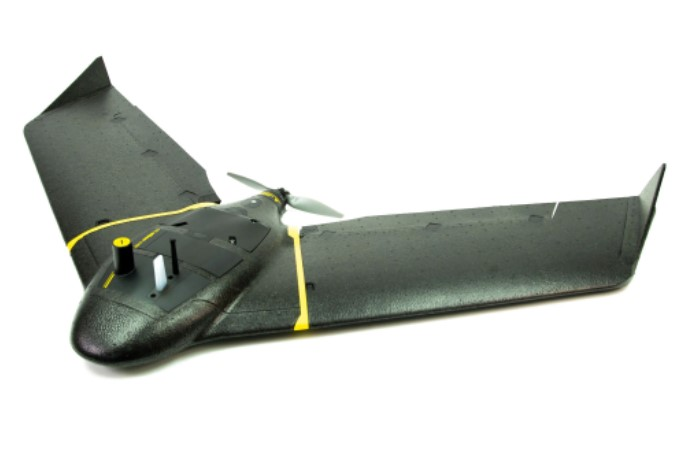
\includegraphics[width=\textwidth]{sensefly-ebee-x.jpg}
        \caption{senseFly eBee X}
        \label{fig:ms-sf-ebee-x}
    \end{subfigure}
    \begin{subfigure}[b]{0.45\textwidth}
        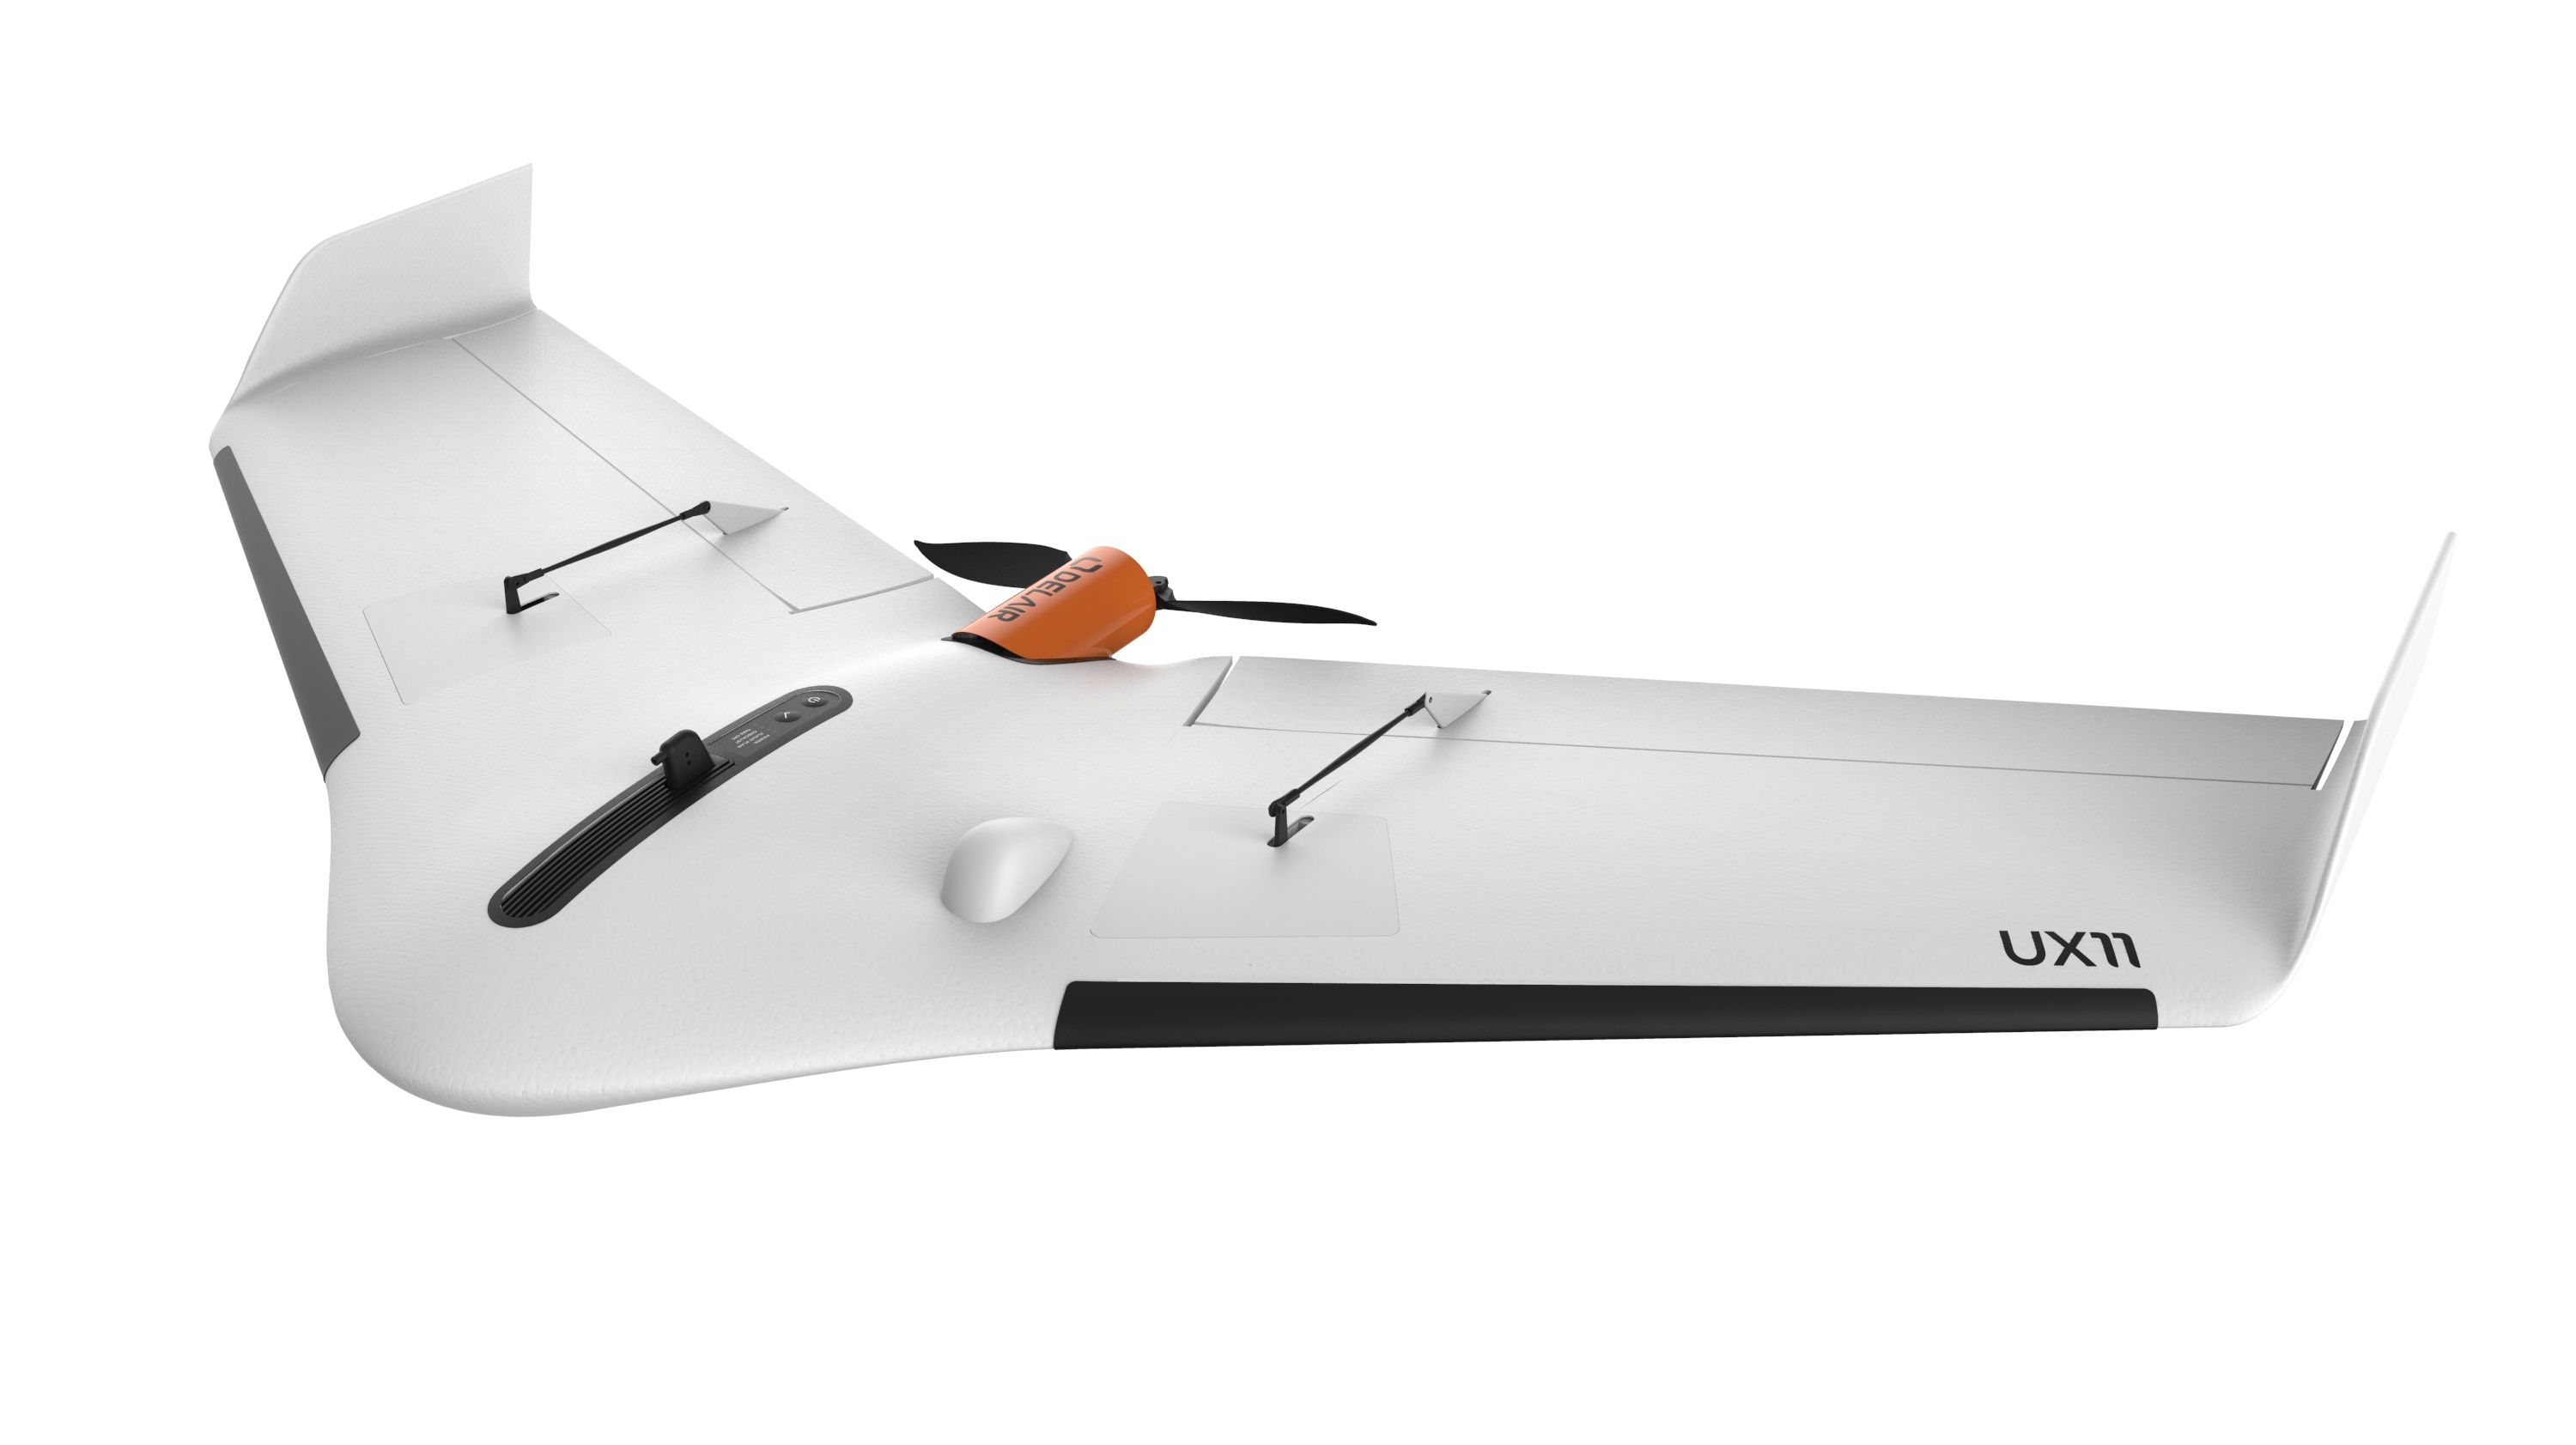
\includegraphics[width=\textwidth]{delair-ux11.jpg}
        \caption{Delair UX11}
        \label{fig:ms-delair-ux11}
    \end{subfigure}
    \begin{subfigure}[b]{0.45\textwidth}
        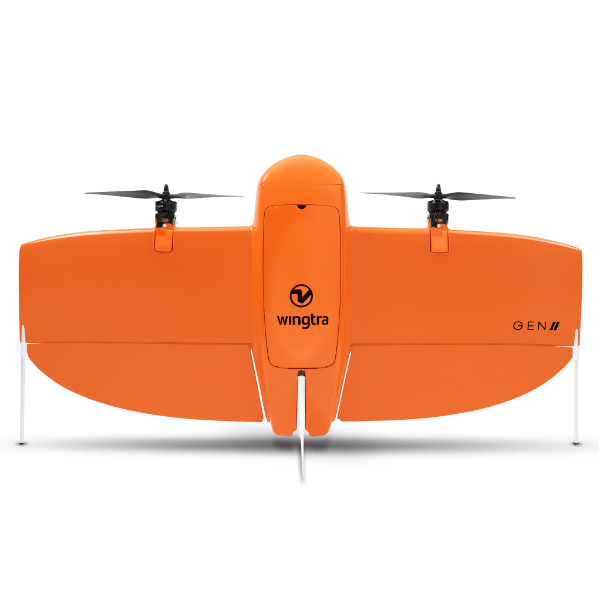
\includegraphics[width=\textwidth]{wingtra-one-ii.png}
        \caption{\href{https://wingtra.com/mapping-drone-wingtraone/}{WingtraOne Gen II}}
    \end{subfigure}
    \begin{subfigure}[b]{0.45\textwidth}
        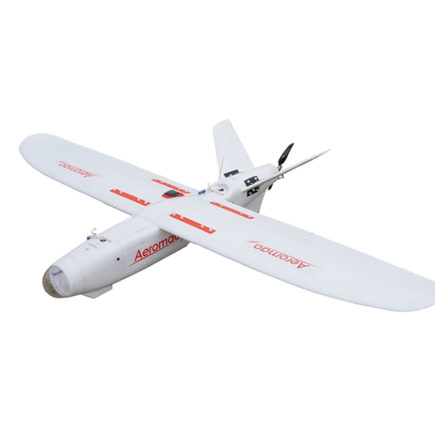
\includegraphics[width=\textwidth]{aeromapper-talon-lite.jpg}
        \caption{\href{https://www.aeromao.com/aeromapper-talon-lite/}{Aeromapper Talon LITE}}
    \end{subfigure}
    \caption{FW-UAV Market Survey}
    \label{fig:market-survey-fwuavs}
    The VTOL capable WingtraOne is also a good choice. Another FW-UAV is Aeromapper Talon LITE
\end{figure}

% Airfoil selection
\subfile{q1-4.tex}

% Components
\subsection{Component Identification}

Identifying all parts of the FW-UAV. The total weight will come around $2\,kg$.

\subsubsection*{Common parts}

The plane \textbf{airfoils} are decided in the previous subsection. We will also need an \emph{aerodynamic body} to join all parts, as well as host all other components.

We will need a \textbf{GPS} module (for location information). We could use the \texttt{NEO-6M GPS Module} (more info \href{https://www.electroschematics.com/neo-6m-gps-module/}{here}).

We will also need two airspeed sensors (mounted in a perpendicular fashion). We could use the \texttt{MATEKSYS Digital Airspeed Sensor (ASPD-4525)} (more info \href{http://www.mateksys.com/?portfolio=aspd-4525}{here}), which will give us the differential pressure (and the airspeed)

We use the \texttt{Ardupilot firmware on BeagleBone Blue} (reference \href{https://ardupilot.org/plane/docs/common-beagle-bone-blue.html}{here}). We can also have a telemetry sensor (or store odometry data on the beagle bone).

We can use the \texttt{EMAX ES08MA II} metal servo (more info \href{https://emaxmodel.com/products/emax-es08ma-ii-12g-mini-metal-gear-analog-servo-for-rc-model-robot-pwm-servo}{here}) for the control surfaces.

\subsubsection*{Propeller, ESC and Battery}

We could use the \texttt{F3P T90-4D} propeller, and the \texttt{AM20 F3P-A} motor \footnote{More about motor \href{http://en.tmotorhobby.com/goods.php?id=1137}{here}, and about propeller \href{https://store.tmotor.com/goods.php?id=1077}{here}}. The ESC can be \texttt{AM66A + AM Link 3D} \footnote{More about the ESC \href{https://store.tmotor.com/goods.php?id=1173}{here}}.

A battery with high enough C rating is needed \footnote{The C Rating gives an estimate of charging and discharging current of a battery $I = C_{r} \times E_{Ah}$. More \href{https://www.power-sonic.com/blog/what-is-a-battery-c-rating/}{here}}. We can choose the \texttt{Turnigy 5000mAh 4S, 20C} battery.

\subsubsection*{Sensor payload}

We can use multiple \texttt{OV2640 Binocular Camera} sensors along with \texttt{Walkera G-2D} gimbal (will require some modifications). This will give high field of view in 3D and require fewer traversals \footnote{More about the camera \href{https://robu.in/product/ov2640-binocular-camera-module-cmos-stm32-driver-3-3v-16001200-for-3d-measurement-with-sccb-interface/?gclid=CjwKCAjwjZmTBhB4EiwAynRmDwSvD0T3b_5tGSfUsN1u4SkNTamfwdZwLdCYZd_c6w4zhIOolFD22hoCSK0QAvD_BwE}{here} and the gimbal \href{http://www.ehirobo.com/walkera-wk-g-2d-brushless-camera-gimbal.html}{here}}.

% Performance analysis and optimization
\subfile{q1-67.tex}
